\section{Analýza matematických modelov}
V predchádzajúcej časti sme spomenuli viacero modelov, ktorými môžeme opísať biochemický reaktor. V tejto časti sa budeme venovať analýze dynamiky a stability dvoch modelov a to Monod modelu doplnenému o produktovú časť a Haldane modelu.

\subsection{Dynamika}
Matematický model, ktorý opisuje biochemický reaktor je nelineárny model. To znamená, že odozva systému je rôzna pre rovnakú veľkosť skokovej zmeny pri rôznych začiatočných podmienkach. Túto nelinearitu si možno všimnúť na Obr. \ref{fig:dyn_monod_ex}. Ten opisuje časový priebeh koncentrácie biomasy, substrátu a produktu Monod modelu pri viacerých skokových zmenách v rýchlosti riedenia. Ďalej si môžeme všimnúť prudký nárast koncentrácie produktu na počiatku, ktorý bol spôsobený nadbytkom biomasy v systéme. Po ustálení dynamika produktu pripomína systém 1. rádu. Na druhej strane v dynamike tvorby biomasy sa prejavuje nestabilná nula (menšie podkmity), ktoré sú spôsobené v dôsledku zvýšenia prietoku látky cez reaktor. Keďže pritečie viac substrátu, čím sa zvýši jeho koncentrácia, koncentrácia biomasy naopak klesne, keďže odtečie viac suspenzie. Následne zvýšená koncentrácia substrátu podporí rast biomasy a tým sa aj koncentrácia biomasy začne zvyšovať. V dynamike substrátu sa zasa prejavuje stabilná nula, ktorá opäť súvisí s väčším prítokom čerstvého média a pomalšou spotrebou substrátu na tvorbu biomasy a produktu.

\begin{figure}
	\centering
	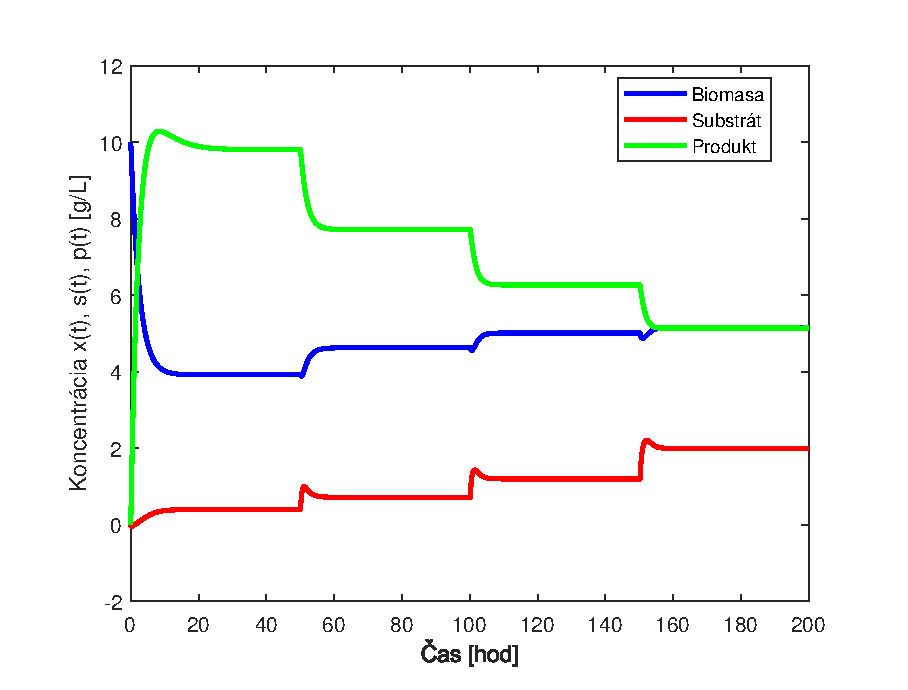
\includegraphics[width=0.7\linewidth]{images/monod_data}
	\caption{Časový priebeh koncentrácie biomasy $ x(t) $, substrátu $ s(t) $ a produktu $ p(t) $ Monod modelu pri viacnásobnej skokovej zmene rýchlosti riedenia $ D = [0.2, 0.3, 0.4, 0.5] $. Parametre modelu: $ \mu_{m} = 0.8\si{\per\hour}, \nu = 0.5\si{\per\hour}, K_{M} = 1.2\si{\gram\per\liter}, Y_{x} = 0.4, Y_{p} = 1, s_{in} = 20\si{\gram\per\liter}, s_0 = p_0 = 0\si{\gram\per\liter} a x_0 = 10\si{\gram\per\liter}$.}
	\label{fig:dyn_monod_ex}
\end{figure}

Režim fungovania biochemického reaktora má významný vplyv na dynamiku celého systému a pri určitých podmienkach Monod model a model s inhibíciou môžu vykazovať rovnaké správanie. Avšak, pri nesprávne zvolených pracovných podmienkach, či už počiatočných podmienkach systému, koncentrácie čerstvého substrátu alebo rýchlosti riedenia, model s inhibíciou bude vykazovať diametrálne odlišné správanie od Monod modelu, ako to je zobrazené na Obr. \ref{fig:dyn_comparison}. Ako môžeme vidieť, zatiaľ čo Monod model sa dostal do nenulového ustáleného stavu, model s inhibíciou klesol s koncentráciou biomasy a produktu na nulu, zatiaľ čo koncentrácia substrátu stúpla na hodnotu 20\si{\gram\per\liter}. Tento stav, kedy reaktorom preteká čistý substrát sa nazýva stav \aps{vymytia} alebo \aps{výplach} a prevádzka reaktora je nenávratne narušená.

\begin{figure}
	\centering
	\begin{subfigure}[b]{0.49\textwidth}
		\centering
		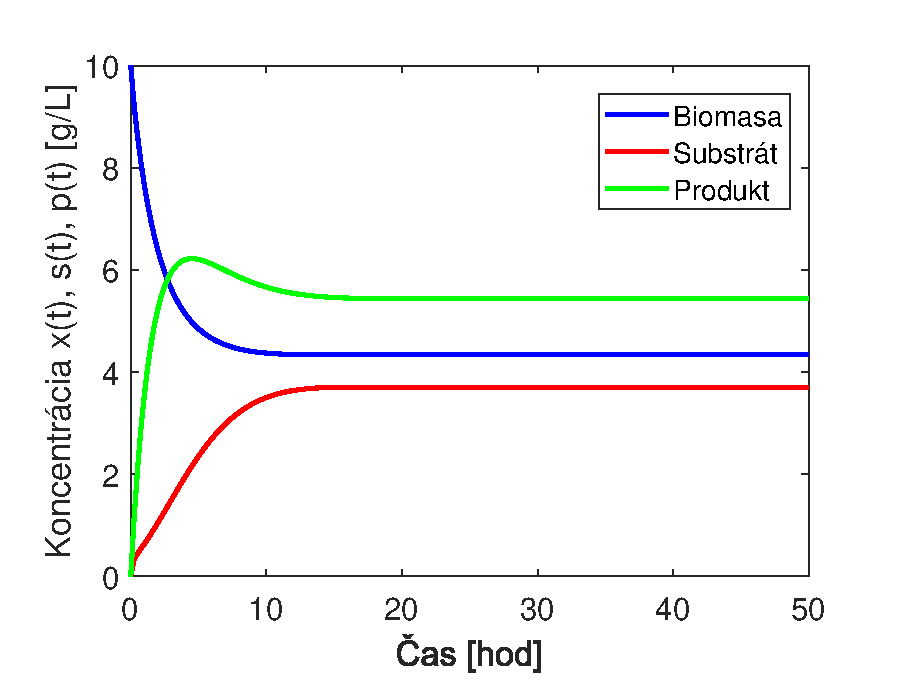
\includegraphics[width=\linewidth]{images/comparison_monod}
		\caption{Monod model}
		\label{fig:dyn_comparison_monod}
	\end{subfigure}
		\begin{subfigure}[b]{0.49\textwidth}
		\centering
		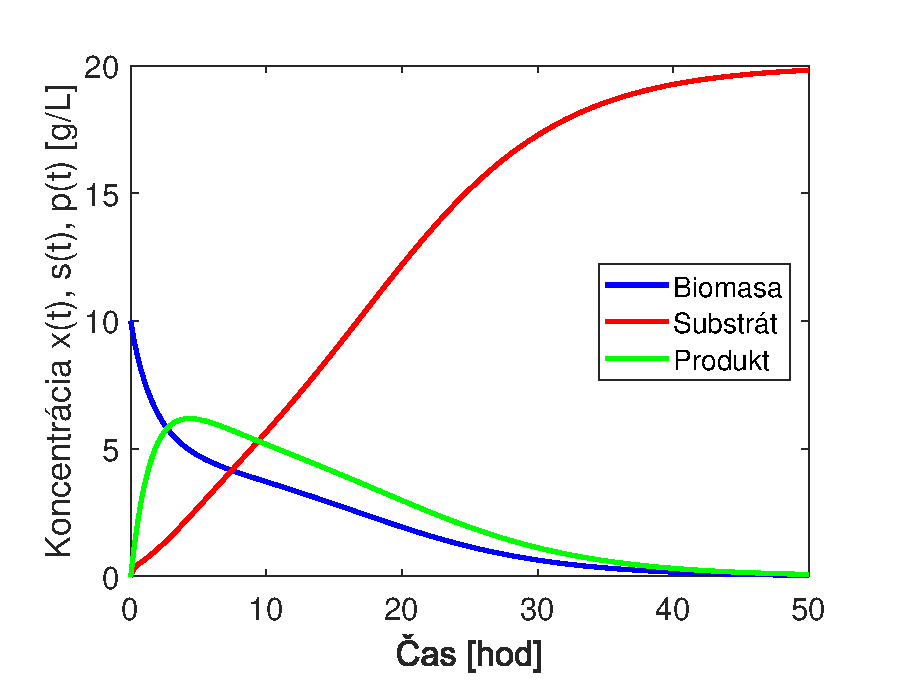
\includegraphics[width=\linewidth]{images/comparison_haldane}
		\caption{Haldane model}
		\label{fig:dyn_comparison_haldane}
	\end{subfigure}
	\caption{Porovnanie dynamiky modelov pri rovnakých pracovných podmienkach. Parametre modelov: $ \mu_{m} = 0.8\si{\per\hour}, \nu = 0.5\si{\per\hour}, K_{M} = 1.2\si{\gram\per\liter}, K_{I} = 20\si{\gram\per\liter}, Y_{x} = 0.4, Y_{p} = 1, s_{in} = 20\si{\gram\per\liter}, s_0 = p_0 = 0\si{\gram\per\liter} a x_0 = 10\si{\gram\per\liter}$.}
	\label{fig:dyn_comparison}
\end{figure}

\newpage
\subsection{Stabilita}
Výhodou prietokových biochemických reaktorov je, že pri dodržaní správnych podmienok, dokážeme systém uviesť do časovo konštantného stavu, ktorý nepretržito pracuje.  Z rovnice \eqref{eq:monod_biomas} vyplýva, že na dosiahnutie ustáleného stavu, je nutné, aby sa buď špecifická rýchlosť rastu rovnala rýchlosti riedenia (takto získame netriviálne riešenie), alebo koncentrácia biomasy je v ľubovolnom čase rovná nule (takto získame triviálne riešenie -- stav vymytia). Ustálené stavy modelov môžeme vidieť na Obr. \ref{fig:spec_rychl_rastu}, ktorý zobrazuje priebeh špecifickej rýchlosti rastu od koncentrácie substrátu pri konštantnej rýchlosti riedenia. Je dobré si všimnúť, že zatiaľ čo Monod model má iba jeden nenulový ustálený stav, model s inhibíciou už obsahuje dva.

\begin{figure}
	\centering
	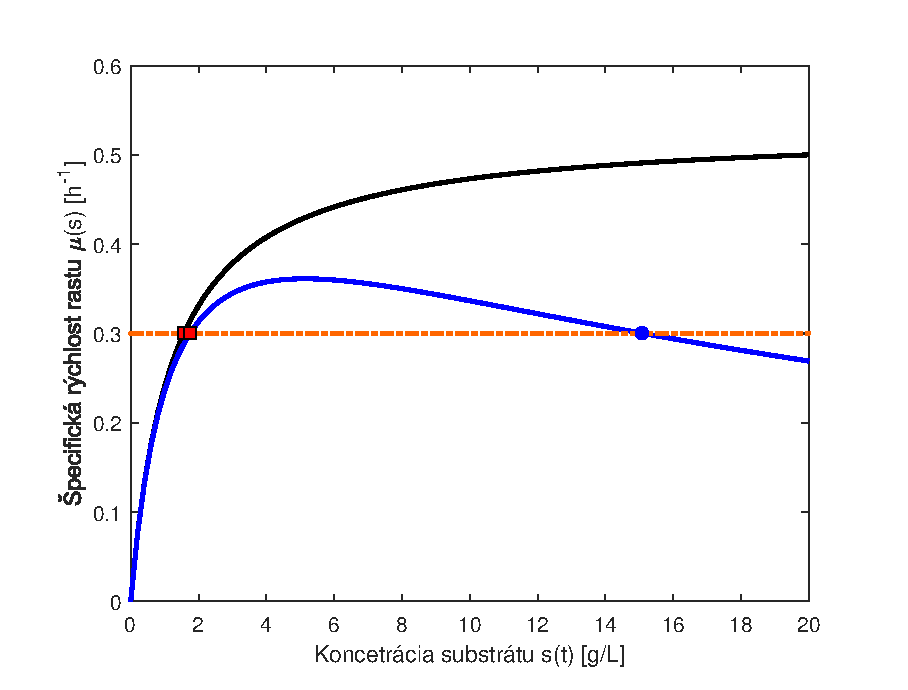
\includegraphics[width=0.7\linewidth]{images/spec_growth_rate}
	\caption{Porovnanie priebehu špecifickej rýchlosti rastu Monod (čierna) a Haldane (modrá) modelu. Zvolená rýchlosť riedenia $ D = 0.33\si{\per\hour} $ (oranžová), stabilné ustálené stavy (červený štvorec), nestabilný stav (modrý krúžok).}
	\label{fig:spec_rychl_rastu}
\end{figure}

\begin{figure}
	\centering
	\begin{subfigure}[b]{0.49\textwidth}
		\centering
		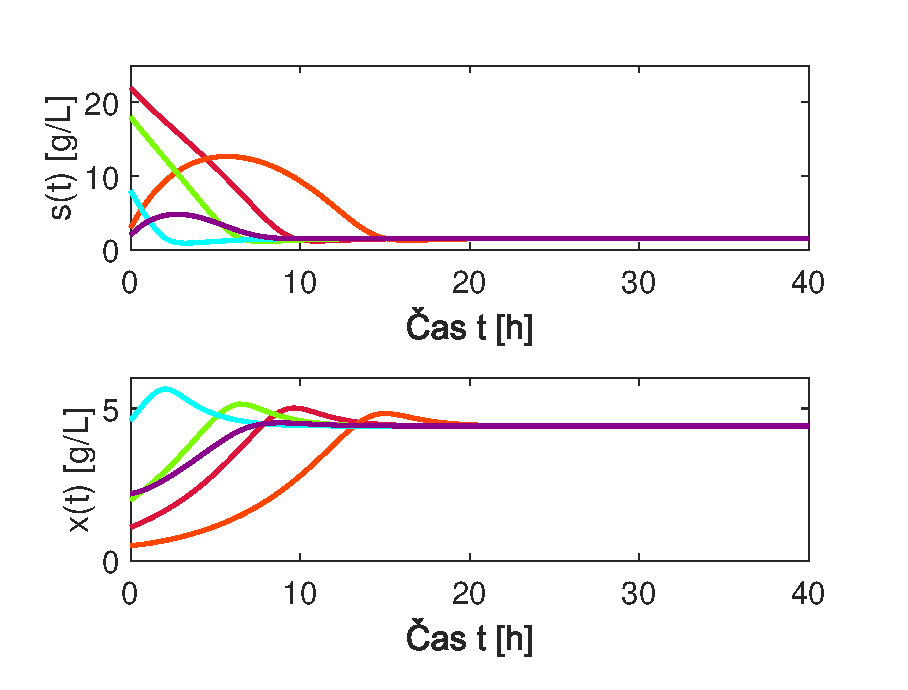
\includegraphics[width=\linewidth]{images/phase1_monod}
		\caption{Časový priebeh koncentrácie biomasy $ x(t) $ a substrátu $ s(t) $.}
		\label{fig:fazovy_vyber_monod}
	\end{subfigure}
	\begin{subfigure}[b]{0.49\textwidth}
		\centering
		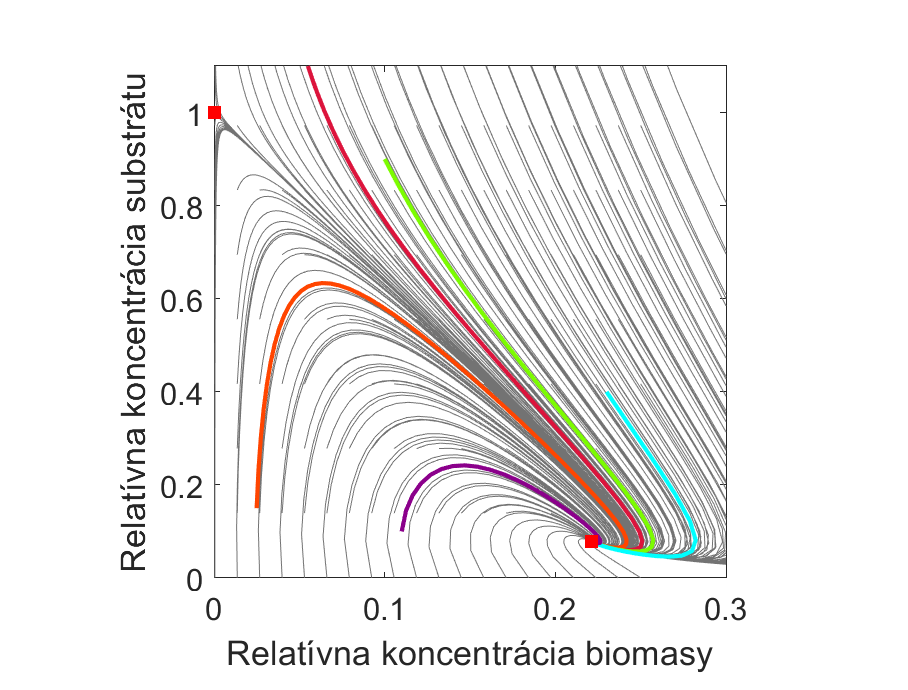
\includegraphics[width=\linewidth]{images/phase2_monod}
		\caption{Fázový diagram. Relatívny pomer vzhľadom na $ s_{in} $.}
		\label{fig:fazovy_monod}
	\end{subfigure}
	\caption{Stabilita a ustálený stav Monod modelu. Nastavenie parametrov modelu: $ \mu_{m} = 0.8\si{\per\hour}, \nu = 0.5\si{\per\hour}, K_{M} = 1.2\si{\gram\per\liter}, Y_{x} = 0.4, Y_{p} = 1, s_{in} = 20\si{\gram\per\liter} $.}
	\label{fig:stabilita_monod}
\end{figure}

Na  fázovom diagrame Monod modelu (Obr. \ref{fig:fazovy_monod}), môžeme vidieť oba ustálené stavy. Ak zvolíme začiatočné podmienky rôzne od nuly (najmä pri koncentrácii biomasy -- vedú k triviálnemu riešeniu a systémom bude pretekať čerstvý substrát) pri konštantnej rýchlosti riedenia menšej alebo rovnej ako špecifická rýchlosť rastu, sa vždy dostaneme do toho istého ustáleného stavu.

\begin{figure}
	\centering
	\begin{subfigure}[b]{0.49\textwidth}
		\centering
		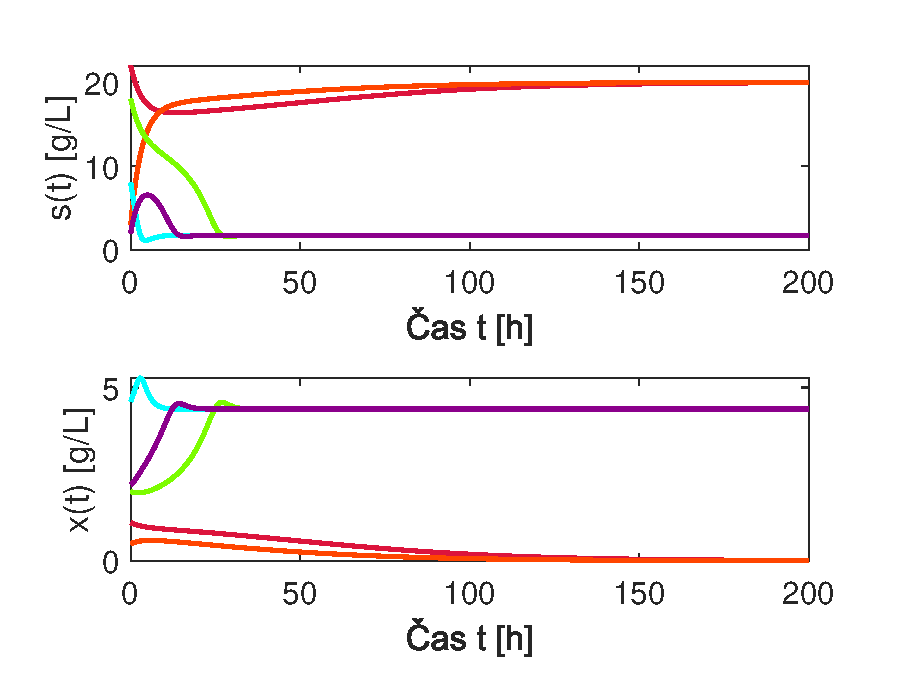
\includegraphics[width=\linewidth]{images/phase1_haldane}
		\caption{Časový priebeh koncentrácie biomasy $ x(t) $ a substrátu $ s(t) $.}
		\label{fig:fazovy_vyber_haldane}
	\end{subfigure}
	\begin{subfigure}[b]{0.49\textwidth}
		\centering
		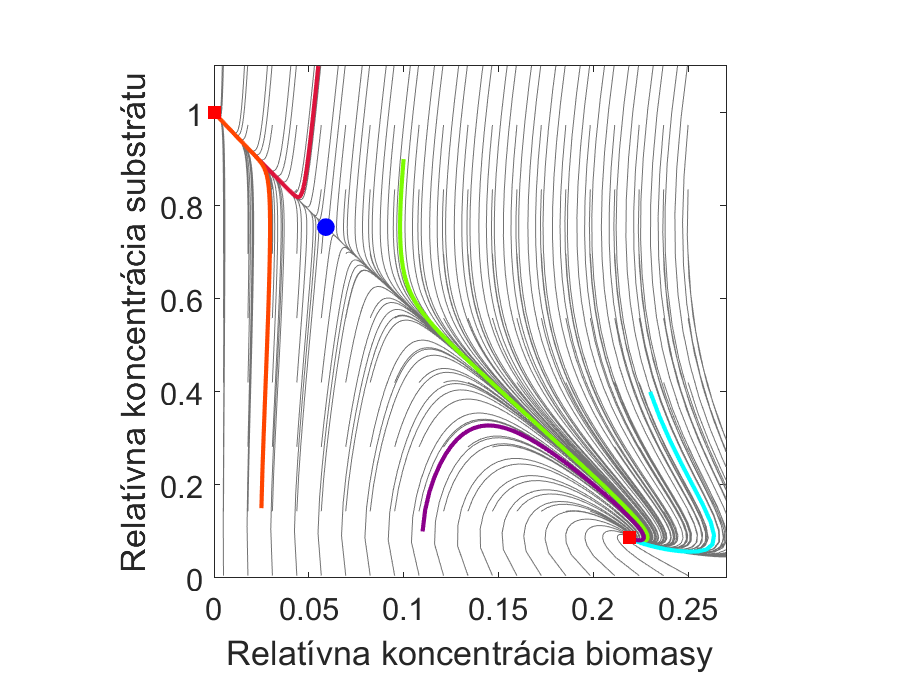
\includegraphics[width=\linewidth]{images/phase2_haldane}
		\caption{Fázový diagram. Relatívny pomer vzhľadom na $ s_{in} $.}
		\label{fig:fazovy_haldane}
	\end{subfigure}
	\caption{Stabilita a ustálený stav Haldane modelu. Nastavenie parametrov modelu: $ \mu_{m} = 0.8\si{\per\hour}, \nu = 0.5\si{\per\hour}, K_{M} = 1.2\si{\gram\per\liter}, K_{I} = 20\si{\gram\per\liter}, Y_{x} = 0.4, Y_{p} = 1, s_{in} = 20\si{\gram\per\liter}$.}
	\label{fig:stabilita_haldane}
\end{figure}

Model s inhibíciou vykazuje odlišné správanie. Na fázovom diagrame (Obr. \ref{fig:fazovy_haldane} napravo) môžeme sledovať už dva nenulové stavy a jeden nulový. Výsledkom triviálneho riešenia je "výplach", ktorý vedie k nulovej koncentrácii biomasy. Ako si môžeme všimnúť, vždy keď je rýchlosť rastu biomasy pomalšia ako je odtok suspenzie zo systému, dostaneme sa do výplachu. Ostali dva netriviálne stavy, z ktorých jeden je nestabilný a druhý je stabilný. V okolí nestabilného stavu môžu nastať dva prípady a to v závislosti od počiatočných podmienok. Ak sa na Obr. \ref{fig:spec_rychl_rastu} nachádzame v okolí nestabilného stavu od neho naľavo, to znamená, že rýchlosť rastu biomasy je väčšia ako odtok suspenzie, dostaneme sa do nenulového ustáleného stavu. Ak sa nachádzame viac napravo, dostaneme sa do výplachu. V skutočnosti by sme to mohli interpretovať aj nasledovne. Ak sa nachádzame v okolí nestabilného stavu naľavo, to znamená, že v dôsledku inhibície nám odumierajú niektoré slabšie mikroorganizmy, ale stále je v systéme dostatok takých, ktoré dokážu znížiť množstvo substrátu v prospech nárastu biomasy a produktu. Tým pádom nám klesne koncentrácia substrátu (pokles koncentrácie substrátu bude sprevádzaný aj poklesom koncentrácie biomasy) a dostaneme sa do stabilného ustáleného stavu. Ak sa však nachádzame napravo od nestabilného stavu, letalita v dôsledku vysokého osmotického tlaku je omnoho väčšia ako vitalita mikroorganizmov a postupne inklinujeme k stavu vymytia.